\label{sec:intro}
Quite often, the evolution of nonlinear systems is well approximated by the nonlinear partial differential equations (PDE). Evidently, there is no universal theory for the solution of nonlinear PDEs, but there exists a distinguished class of nonlinear equations that can be solved with a mathematical rigour: the so-called \textit{integrable systems}. The history of integrable PDEs started in the 1960s when Gardner et al. \cite{ggk67} discovered a method for finding the infinite families of exact solutions for the  Korteweg-de Vries equation. Their method termed the inverse scattering transform, can be deemed as the generalisation of the conventional Fourier transform (FT) to the nonlinear systems. Thus, the name nonlinear Fourier transform (NFT) for it is often used nowadays, especially in the signal processing literature \cite{yk14-1,tplwfkd17}. Shortly after the integration of the Korteweg-de Vries equation, Zakharov and Shabat developed the inverse scattering machinery (i.e. the NFT method) for yet another celebrated PDE: the nonlinear Schr\"odinger equation (NLSE) \cite{zs72}, which will be the focus of our current study.  

In a nutshell, for an integrable PDE there exists the canonical transform of dependent variables, converting the original nonlinear system into the so-called action-angle variables; the evolution of the latter is governed by a set of uncoupled trivial (linear) differential equations. Mathematically, this can be treated as the effective linearisation of a nonlinear integrable PDE \cite{akn74,nmp84}. For our work, it is important that we know the explicit form of the NFT operations attributed to the NLSE.

The NLSE, being a generic model describing the interplay between the dispersive and nonlinear effects, is applicable to the description of a vast number of physical phenomena, ranging from the dynamics of magneto-ordered systems \cite{kik90} to hydrodynamics \cite{o10}. It also serves, under certain assumptions, as a principal master model governing the evolution of a single-polarisation slow-varying light envelope propagating along the single-mode fibre \cite{a12,mg06}. In the dimensionless form we write down the NLSE as: 
\begin{equation}
i \frac{\partial q}{\partial z} + \frac{1}{2}\,\frac{\partial^2 q}{\partial t^2} + |q|^2 q = 0 ,
\label{NLSE-in}
\end{equation}
In the fibre-optic context, $q(z,t)$ is the electromagnetic field evolving down the fibre, $z$ is the distance along with the fibre, while $t$ is the retarded time variable. Eq.~(\ref{NLSE-in}) is explicitly written as the focusing NLSE, corresponding to the anomalous dispersion of the standard optical fibre. We note that our further results are general and can be used for various physical applications, where NLSE~(\ref{NLSE-in}) provides a good approximation. Nonetheless, without loss of generality, we will refer in the paper to the field $q$ as to ``a signal''.

Withing modern optical communications, the NFT is used not as a tool for the NLSE solution, but as a signal processing method \cite{tplwfkd17,yk14-1}. This concept originated from the work of Hasegawa and Nyu \cite{hn93}, who proposed to depart from considering the time domain solitonic shapes \cite{mg06}, but rather use the nonlinear spectrum (the so-called eigenvalues) for the data modulation and transmission. Over the last decade, the NFT-based optical transmission techniques have been resurrected and greatly extended~\cite{tplwfkd17,yal19}. The most efficient NFT-based optical transmission method is the so-called nonlinear frequency division multiplexing (NFDM) \cite{yk14-1}, within which we directly modulate the parameters of the nonlinear modes that emerge from the nonlinear Fourier (NF) signal decomposition. When the optical field propagates down the fibre link, the evolution of the nonlinear modes inside the NF domain stays almost linear, in contrast to the truly nonlinear evolution of signal in the space-time domain. Due to this property, we can theoretically get rid of the infamous nonlinear cross-talk degrading the transmission performance at high signal powers\cite{ekw10}. 

Generally, when considering the NF decomposition of an arbitrary rapidly decaying wave-form, we can have two distinct coexisting parts of the NF spectrum: the continuous part, describing quasi-linear dispersive waves, and the discrete part, corresponding to solitonic modes \cite{nmp84,akn74,tplwfkd17,yk14-1}. The continuous part of NF spectrum is represented by the complex-valued function $r(\xi) \in \mathbb{C}$ of a real argument $\xi \in \mathbb{R}$, where $\xi$ is called the spectral parameter; $r(\xi)$ is called the reflection coefficient, and $\xi$ emerges as the nonlinear analogue of a conventional Fourier frequency. This NF spectrum part converges to the conventional FT of our signal in the low-power limit \cite{pdt13}, see also the explicit expressions in Methods. The discrete part consists of the complex eigenvalues $\xi_n \in \mathbb{C}^{+}$, located in the upper complex half-plane, and the associated norming constants $r_n$ (spectral amplitudes) \cite{a16}. The graphical summary of the general NF spectrum structure is given in Fig.~\ref{fig:spectrum_representation}. However, we point out that it is exactly the utilisation of the \textit{continuous NF spectrum part} \cite{pdbgt14,lpt14,lpt15,lpr15,lpphet16,lab17,kplt17_2,yy19} that resulted in the breakthrough in the NFDM technology: this idea, mentioned already in early NFT transmission-related works \cite{yk14-1,pdt13}, is in stark contrast with the progenitor soliton-based transmission methods~\cite{mg06}. In our current study we specifically address the continuous NF spectrum: our goal is to compute the profile $r(\xi)$ given the localised $q(t)$ shape. Then, we mention that the continuous NF spectrum modulation using the special technique coined b-modulation \cite{w17,gzl18,svp20,cw20} has provided the highest NFDM data rates so far \cite{yal19,yla19}. Thus, in this paper we also address the recovery of the b-coefficient, $b(\xi) \in \mathbb{C}$, $\xi \in \mathbb{R}$, given $q(t)$. When the solitons are absent, as it is in the case considered, the full NF spectrum corresponding to a given finite-extent signal can be equivalently represented by either the reflection coefficient or by the b-coefficient, see more in Methods. Finally, we note that for the NFDM based on the discrete NF spectrum \cite{hyk16,bai16,wxz20}, the achieved data rates have been noticeably lower than those for the modulation of continuous NF spectrum, see the comparison in \cite[Fig. 1]{yal19}, and we do not address the computation of solitonic parameters in our research.
\begin{figure}[tbh]
    \centering
    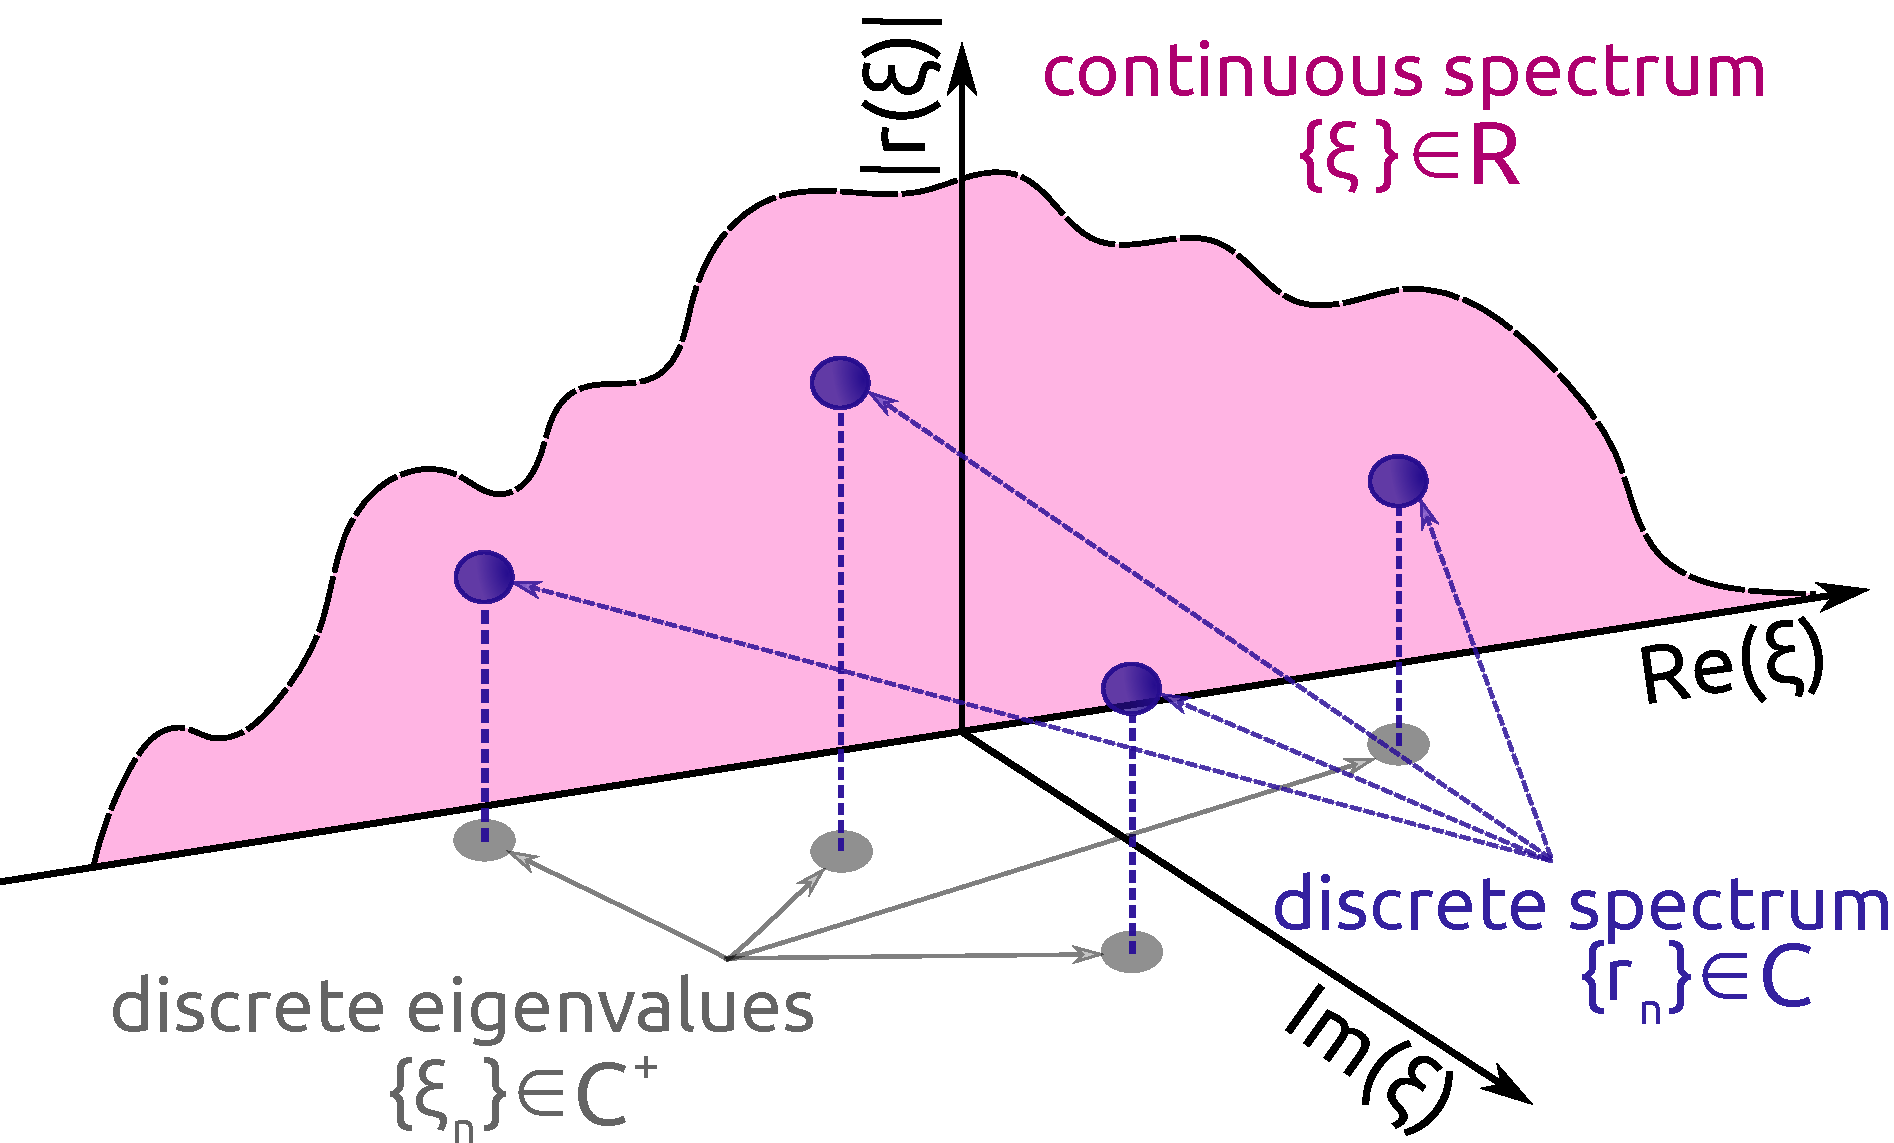
\includegraphics[width=0.55\linewidth]{images/nn_nft/nft_spectrum_representation_6.pdf}
    \caption{The schematic showing the different coexisting parts of a general NF spectrum: the discrete part, represented by the eigenvalues $\xi_n$ and respective norming constants $r_n$, and the continuous part, shown as the function $|r(\xi)|$ on the real $\xi$-axis. }
    \label{fig:spectrum_representation}
\end{figure}


The NFDM transmission method relies on the (approximate) integrability of our transmission channel, i.e. we inherently assume that Eq.~(\ref{NLSE-in}) is a very accurate model describing the signal evolution down the fibre. However, aside from second-order dispersion and Kerr nonlinearity present in (\ref{NLSE-in}), in realistic fibre-optic systems, there are numerous other effects affecting signal's propagation. Optical noise inevitably arising during the amplification process \cite{a12} is one of the key challenges in optical communications. The noise results in random NF spectrum disturbances \cite{dpt16,pvd20}, imposing limits on the NFDM transmission quality. Thus, in our current work, we analyse the capability of a neural network (NN) to denoise the NF spectra. Another widespread deviation from idealised model (\ref{NLSE-in}) is the non-zero nonuniform gain-loss profile occurring in realistic systems for both lumped \cite{lpt15,kplt17_2} and distributed \cite{lpr15} amplification schemes. We also mention the effects of polarisation mode dispersion \cite{ylb17,ts19}, higher-order chromatic dispersion \cite{ylb17}, and component-induced impairments, to itemise just several important sources. All these effects bring about the deviations of the true optical channel from integrable NLSE (\ref{NLSE-in}) such that the NF spectrum of the signal at the end of our transmission system can be significantly distorted, which results in the appearance of errors in the transmitted data \cite{lpphet16,lab17,ylb17}.  Given that,  the machine learning and artificial neural networks (NN) based signal processing methods have recently attracted much attention, as they can effectively render adaptive distortions-resilient signal processing tools, and, thus, using the NNs we can mitigate the impact of detrimental factors mentioned above \cite{mrn18,kfl19}.  


The first direction of utilising NNs for NFDM systems consists in applying the additional NN-based processing unit at the receiver to compensate the emerging line impairments and deviations from the ideal model \cite{gdd18,kwp19,kkp19,kpk20,kkp21}. But, despite ensuing transmission quality improvement, this type of NN usage brings about the additional complexity of the receiver. In the other approach, the NFT operation at the receiver is entirely replaced by the NN element. It has been shown that this approach, indeed, results in a considerable improvement of the NFT-based transmission system functioning \cite{ymm19,jgy18,wxz20}. But, despite the benefits rendered by such a NN utilisation, the NNs emulating the NFT operation have so far been mostly used in the NFDM systems operating with solitons only, and the NN structure used there was relatively simple.  In the only work related to the continuous NF spectrum recovery~\cite{zhang2021direct}, a standard ``imageInputLayer'' NN (developed originally for hand-written digits recognition) from MATLAB 2019a deep learning toolbox was adapted to process the signals of a special form. Such an approach, evidently, has limited applicability and flexibility and is not optimal neither in terms of the result's quality nor in the complexity of signal processing. 
In our current work, we demonstrate how this direction can be significantly extended and optimised, presenting and analysing the NN-based NFT modelling for the continuous NF spectrum, and using the special optimisation tools for finding the best NN architecture. We believe that our current research can lay the basis for the development of high-efficiency channel-agnostic NFDM transmission systems. Moreover, in our study, we address the question of recovering not only the NF spectrum $r(\xi)$, but also the b-coefficient, so it can be combined with the most efficient NFDM transmission method: the b-modulation.

Finally, we note that, recently, the interest in using the NFT as a signal-processing tool has risen in fields that are not directly relevant to optical transmission. In particular, the NFT was applied in the so-called integrable turbulence to monitor the appearance of coherent structures, such as breathers, solitons, and rogue waves \cite{rsc18,sda16}, to the optical microresonators regime analysis \cite{tcf20}, to the optical frequency combs characterisation \cite{wsh20}, and to the analysis of laser regimes and the emergence of dissipative coherent nonlinear structures \cite{rnb18,skp19,csf19}. The analysis of NFT modes' evolution for such systems often appears to be more informative and convenient than dealing with the conventional Fourier modes. The NFT is also an important tool for the design of fibre Bragg gratings \cite{FBG01,FBG02}. Thus, we believe that the technique presented in this work can have a much wider range of applications than simply being a processing tool in optical communications. To end up, solving nonlinear differential equations itself by using NNs is a fast-growing area with a range of applications in science and engineering \cite{rbp17,lkb18,lka20}. We hope that our work will also advance knowledge in this emerging field.
